
% C.5.2 - The Interferential Tensor Field: Phase Coherence and Structural Projection
\section*{C.5.2 The Interferential Tensor Field: Phase Coherence and Structural Projection}

\subsection*{1. Tensorial View of Interference}
In Kasoku Theory, interference is not merely the summation of wave amplitudes but the active structuring of space-time density through dynamic fluctuations known as Kasoku. These fluctuations are inherently directional, non-symmetric, and collectively generate phase structures of varying coherence. To represent this multidimensional structure, we introduce the \emph{Kasoku Interference Tensor Field}.

\begin{figure}[h!]
\centering
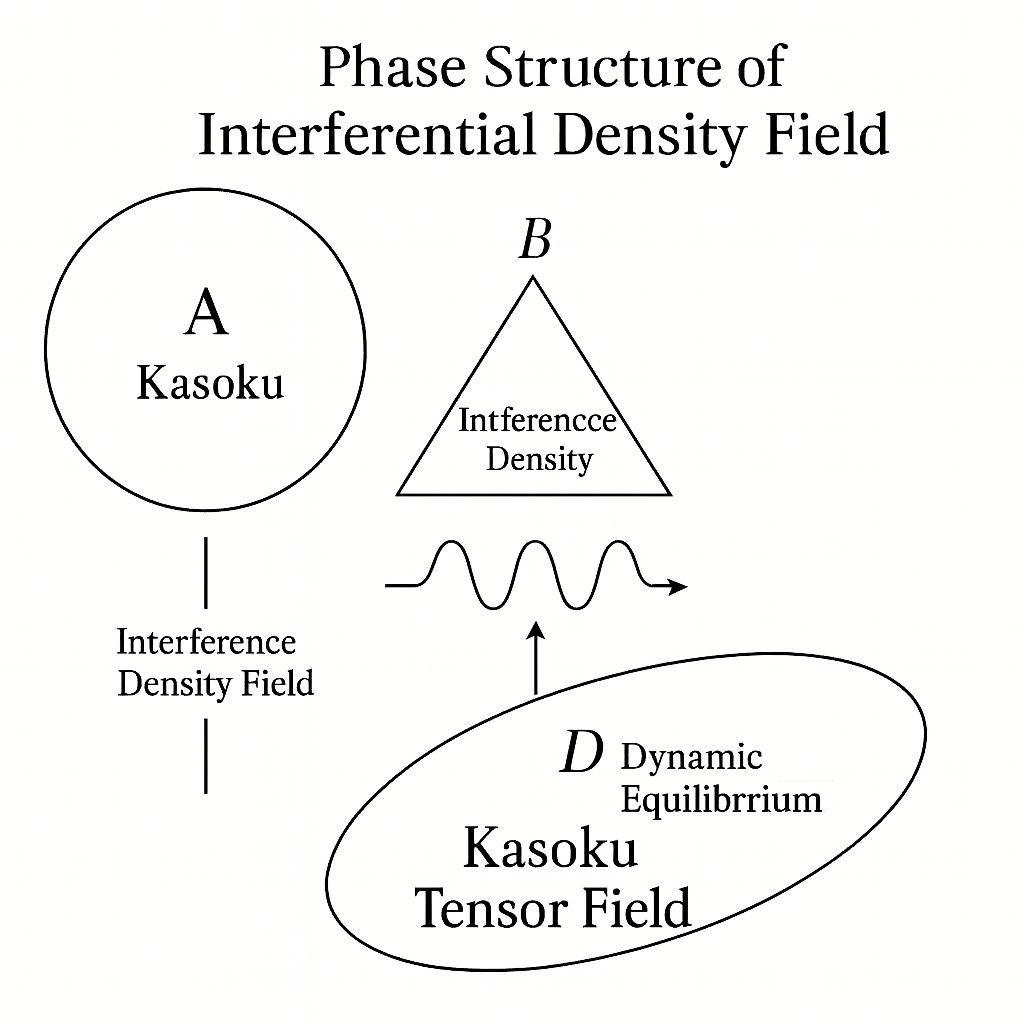
\includegraphics[width=0.7\textwidth]{Phase Structure of Interferential Density Field.png}
\caption{Visual representation of phase density structures created by directional Kasoku interference. This diagram illustrates the evolving topology of coherence and local deformation within the field.}
\end{figure}

\subsection*{2. Definition of the Interference Tensor \( T_{\mu\nu} \)}
We define a second-rank tensor field \( T_{\mu\nu}(x,t) \) that captures the directional correlation of interference fluctuations:
\[
T_{\mu\nu}(x,t) = \sum_{i,j} \langle \delta_\mu^{(i)} \delta_\nu^{(j)} \cdot I(x,t) \rangle
\]
Here, \( \delta_\mu^{(i)} \) represents the \( \mu \)-axis component of the \( i \)-th Kasoku vector at position \( x \) and time \( t \), and \( I(x,t) \) is the local interference density.

- The \textbf{diagonal components} \( T_{\mu\mu} \) reflect the intensity of fluctuations in each direction.
- The \textbf{off-diagonal components} \( T_{\mu\nu} \) (for \( \mu \ne \nu \)) measure cross-directional coupling — i.e., \emph{structural twisting} or "creases" in the interference field ("hidas").

\begin{figure}[h!]
\centering
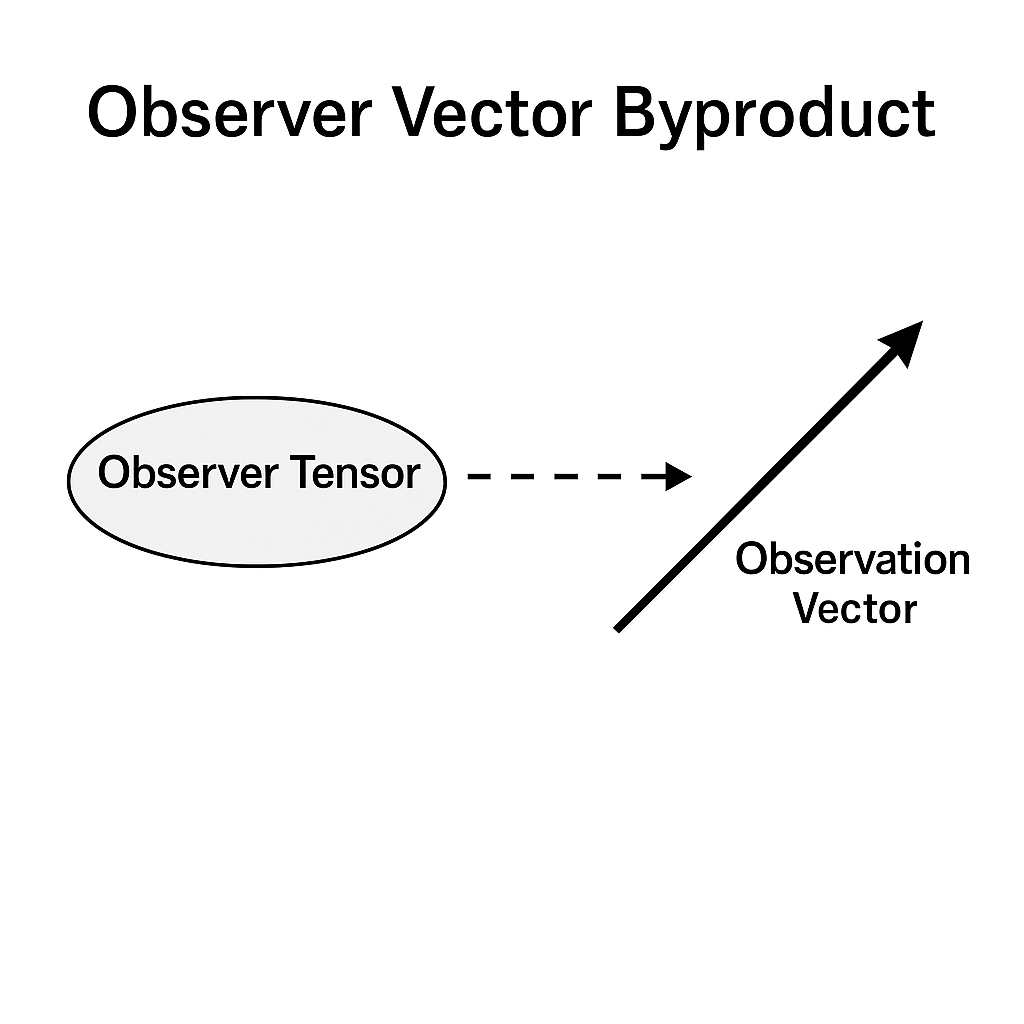
\includegraphics[width=0.65\textwidth]{Observer Vector Byproduct.png}
\caption{Schematic showing the observer effect: once a Kasoku vector is fixed through observation, a residual directional byproduct emerges. This diagram highlights the philosophical asymmetry introduced by observational collapse.}
\end{figure}

\subsection*{3. Scalar Metrics: Coherence \( \mathcal{C} \) and Entropy \( S \)}
To evaluate the structural alignment of the field, we introduce two scalar indicators:

\paragraph{(a) Coherence \( \mathcal{C}(x,t) \)}
\[
\mathcal{C}(x,t) = \frac{|\sum_i \Psi_i(x,t)|^2}{\sum_i |\Psi_i(x,t)|^2}
\]
This metric reflects the degree of phase alignment. \( \mathcal{C} = 1 \) implies perfect constructive interference; \( \mathcal{C} = 0 \) indicates complete phase incoherence.

\paragraph{(b) Kasoku Entropy \( S_{\text{Kasoku}} \)}
\[
S_{\text{Kasoku}} = -\sum_{\theta} p(\theta) \log p(\theta)
\]
Where \( p(\theta) \) denotes the angular distribution probability of Kasoku directions. Higher entropy indicates a more disordered phase field.

\subsection*{4. Interpreting the Tensor Field}
The interplay between \( T_{\mu\nu} \), \( \mathcal{C} \), and \( S \) reveals a rich geometry of phase structures:

- High coherence corresponds to low entropy and minimal off-diagonal tensor values.
- High off-diagonal values correlate with complex “creases” and increased disorder.

These relationships imply that interference structures can be mapped, tracked, and potentially classified by their tensorial signature — allowing a new form of structural spectroscopy.

\subsection*{5. Third-Rank Tensors and Triadic Interference Colonies}
To capture more complex phase entanglement, we extend the tensor field to rank three:
\[
T_{\mu\nu\lambda}(x,t) = \sum_{i,j,k} \langle \delta_\mu^{(i)} \delta_\nu^{(j)} \delta_\lambda^{(k)} \cdot I(x,t) \rangle
\]
This third-rank tensor encodes triplet-wise directional interference — the minimal unit of a structural “crease” that cannot be decomposed into purely pairwise interactions. It serves as a descriptor of localized resonance colonies: triangular feedback loops, vortex crossings, or seed-like honeycomb curvatures.

The mathematical structure \( T_{\mu\nu\lambda} \) may allow us to model:
\begin{itemize}
    \item \textbf{Triadic Resonance Conditions}: where three Kasoku vectors reinforce a local fold.
    \item \textbf{Curved Phase Seeds}: capturing early-stage bubble-like nucleation of spatial domains.
    \item \textbf{Fractal Hida Chains}: recursive generation of crease networks through third-order coupling.
\end{itemize}

\begin{figure}[h!]
\centering
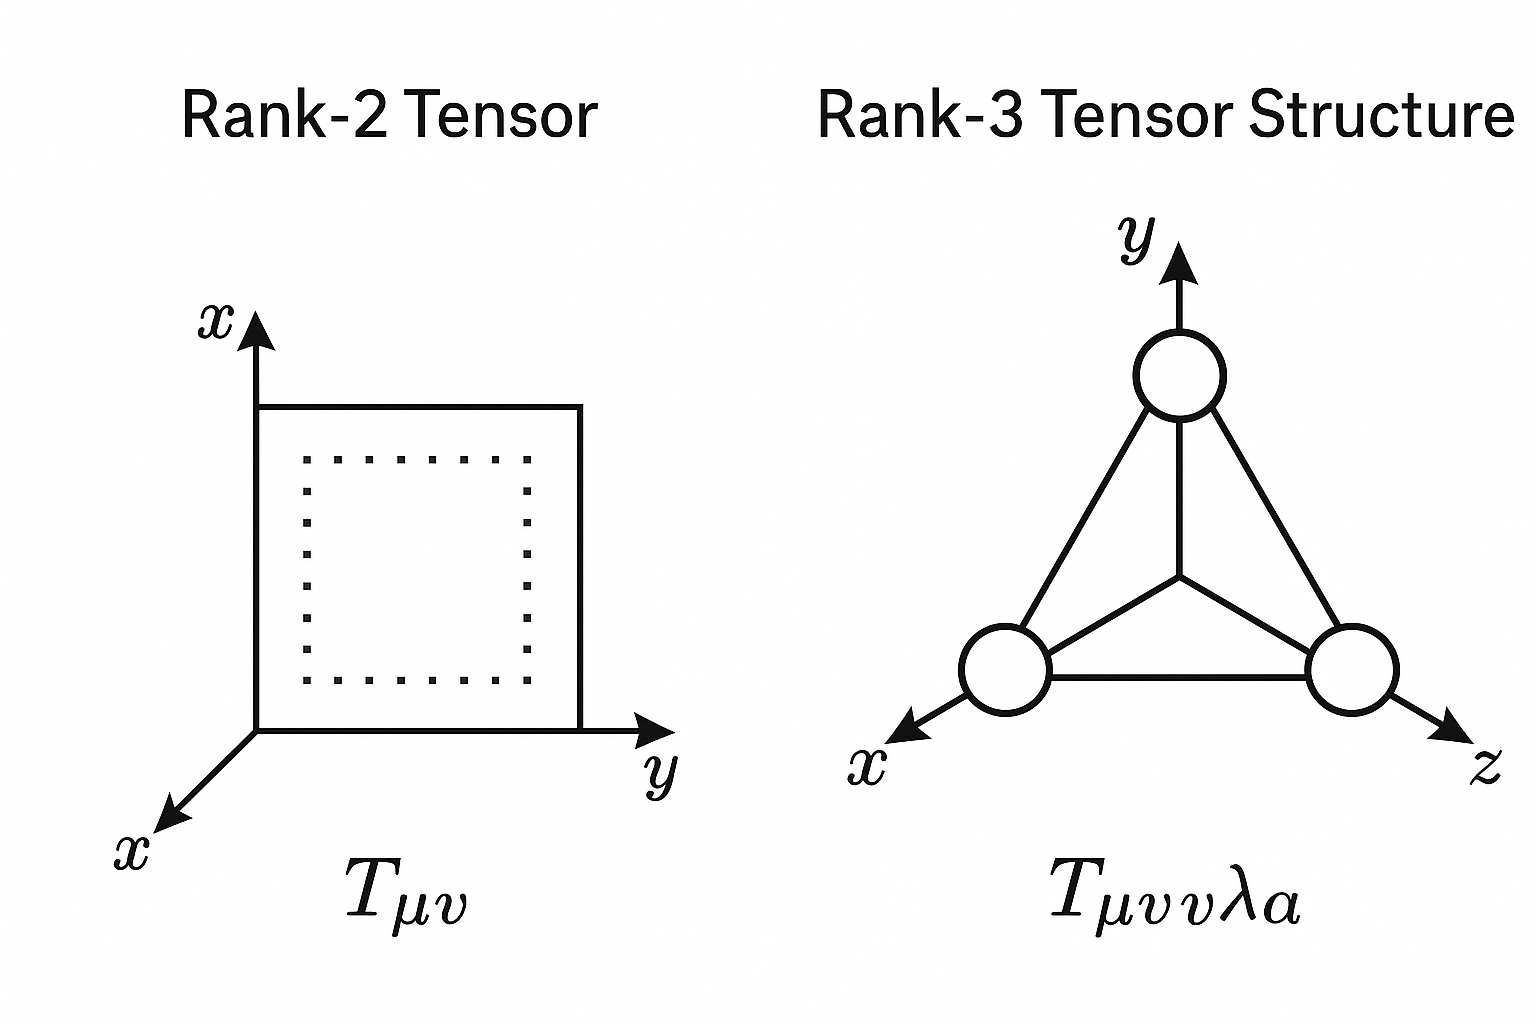
\includegraphics[width=0.72\textwidth]{Triadic Interference Tensor Structure.png}
\caption{Conceptual visualization of third-rank interference tensor \( T_{\mu\nu\lambda} \) representing phase-triplet entanglement. Local resonance colonies emerge from coherent triangular interference structures.}
\end{figure}

\subsection*{6. Philosophical Note: Ethics of Observation}
Observation, in this framework, acts as a projection — collapsing a dynamic field into fixed meaning. This collapse eliminates unchosen pathways, forming what we call \textit{meaning-death}. For further treatment, see Supplement C.5.4a: \emph{Observation as Structural Collapse}. The act of interpreting the tensor field is thus not neutral, but participatory — imbued with both structural and ethical implications.
